%%%%%%%%%%
% [TODO] %
%%%%%%%%%%
% [ ] Mini-intro
% [ ] surfphono
% [ ] k-epenth
% [ ] Mini-discussion

%%%%%%%%%%%%%%%%%%%%%%
% Chapter mini-intro %
%%%%%%%%%%%%%%%%%%%%%%

%%% Short BG
%\subsection{ASR tools as models of perception}


%%% Research question + alternatives


%%% Plan


%%%%%%%%%%%%%%%%%%%
% General methods % %
%%%%%%%%%%%%%%%%%%%

\section{Anatomy of our HMM-based speech recogniser}
For the experiments described in this chapter we used Hidden Markov Model (HMM)-based speech recognisers as models of human perception. 
Speech audio waveforms are transformed into a sequence of \textbf{acoustic vectors} $X_{1:T} = x_{1}, ..., x_{T}$ through the first step, called feature extraction. In the decoding phase that follows, the trained ASR system attempts to find the sequence of words $w_{1:L} = w_{1}, ..., w_{L}$ which is most likely to have produced the sequence of acoustic feature vectors $X$.
Mathematically, this equates to solving the following equation:

\begin{equation}
  \widehat{w} = \underset{w}{arg\,max} \left \{  P(w|X)\right \}
  \label{eq_hmm_dec_post}
\end{equation}

Put into Bayesian terms, this represents computing the posterior probability $P(w|X)$ of all combinations of words, given the acoustics, and retrieving the index of the most probable one: the decoder selects the sequence of words $w$ with highest posterior probability given the acoustic evidence $X$. However, due to the fact that there is an infinite number of possible combinations of words, it may be difficult to evaluate all possible combinations in order to find the most probable one. As such, following Bayes's theorem, equation \ref{eq_hmm_dec_post} can be rearranged as:

\begin{equation}
  \widehat{w} = \underset{w}{arg\,max} \left \{  P(X|w)P(w)\right \}\footnote{In practice $P(X|w)P(w)$ is often computed in the log space as $\alpha ~log P(X|w) + log P(w)$, where $\alpha$ is a scaling factor called acoustic scale (set to $0.1$ in our models)}
  \label{eq_hmm_dec_post}
\end{equation}
The likelihood $P(X|w)$, given by the \textbf{acoustic model}, is the probability of the acoustics given the sequence of words. The prior $P(w)$, given by the \textbf{language model}, corresponds to the probability of the word sequence, and can be derived from frequency counts. These probabilities can be extracted by training our ASR system using annotated speech corpora.

Nowadays, in the field of ASR, Neural Network (NN)-based speech recognisers are the state-of-the-art. In spite of better performance of NN-based ASR systems, we decided to use HMM-based recognisers, which are better understood than NNs while still offering good speech recognition performance. Indeed, before the decoding step, these models offer a clear separation between the acoustic model (AM; i.e., mapping between phoneme categories and acoustics) and the language model (LM; i.e., frequencies of word/phoneme sequences). This allowed us to test ASR systems with different LMs while keeping the AM constant, as well as adapting LMs to mimic the experimental paradigms used when testing human participants. Importantly, unlike NNs which are often qualified as ``black boxes'', we are able to better understand and analyse how the ASR system processes acoustic input. 
We will now present the necessary components for building an HMM-based ASR system, namely the speech corpora used to train and test the system and its featural representation, as well as the decoder itself, composed of an acoustic model, a lexicon, and a language model. The interaction of these elements is depicted in Figure \ref{fig:hmm_architecture}. In the following subsections we will present the components in more detail. 

\begin{figure}[htb]
\centering
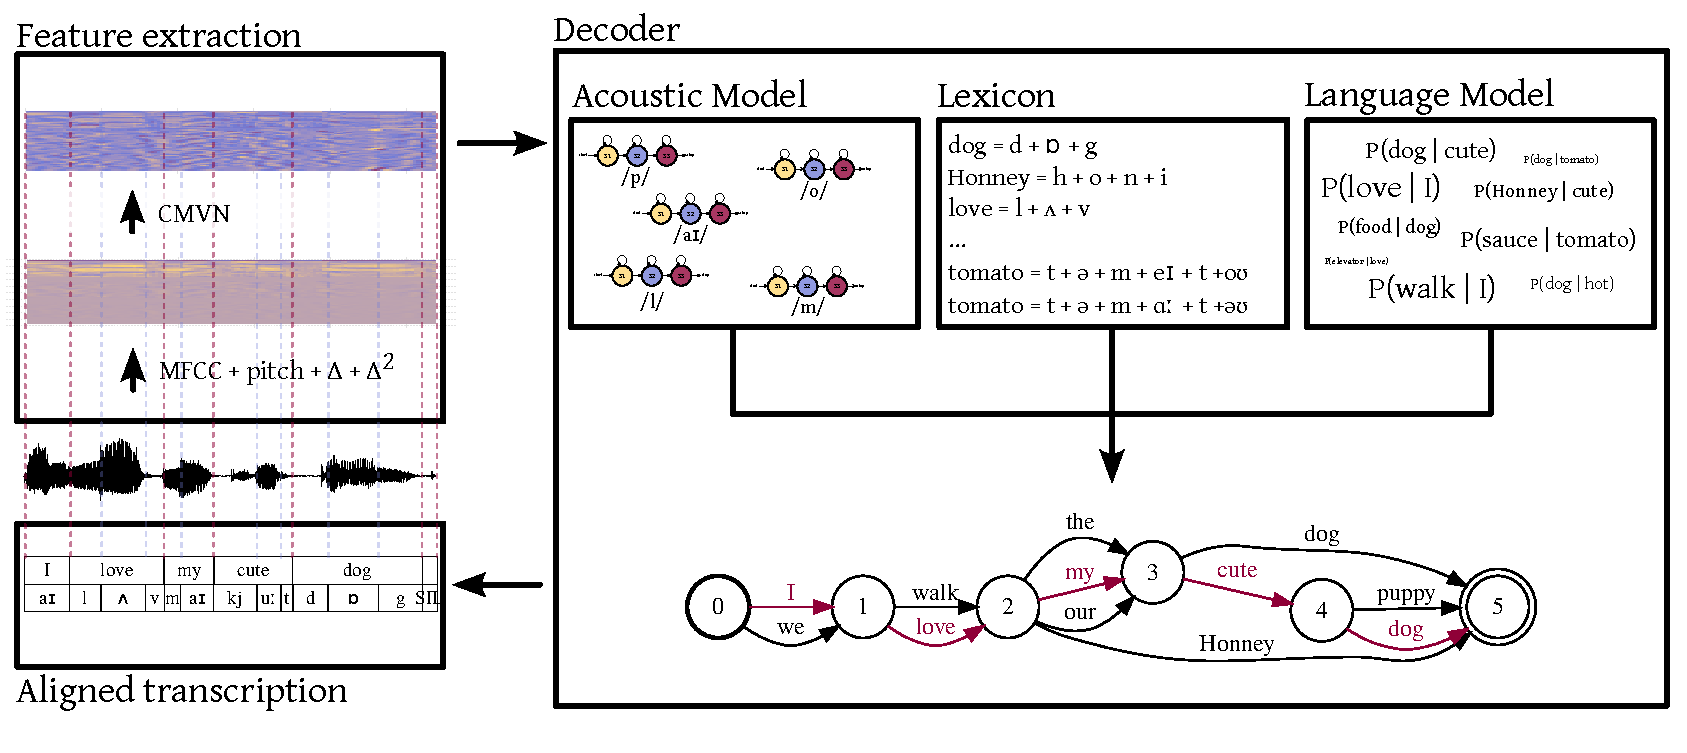
\includegraphics[width=1\linewidth]{chapter03/hmm_all_version2.pdf}
\caption{\textit{Architecture of our ASR system, including its input (acoustic features) and output (transcription).}}
\label{fig:hmm_architecture}
\end{figure}

\subsection{Corpora}

In order to train and test our ASR system, we required transcribed speech corpora. These corpora consisted of speech recordings which have been annotated; for each utterance, we have a more or less detailed transcription of what was said.
While the ideal annotation is one for which phoneticians have provided phoneme categories (or even phones), as well as their boundaries, often we might only have access to by-utterance annotations where we are only provided with a sequence of words/phonemes for each utterance. In these cases, we rely on forced alignment to automatically find phoneme boundaries.

In the following sections we have trained ASR systems with different ``native'' languages, namely Japanese (JP) and Korean (KR). These languages were of particular interest because of their relatively restrictive phonotactics with regards to consonant clusters, as well as the availability of corpora of spontaneous speech, which we will now present. We also trained an American English (EN) corpus in order to evaluate our model's performance with respect to state-of-the-art systems. 

\paragraph{Corpus of Spontaneous Japanese (CSJ)}
As the name suggests, the CSJ \cite{maekawa2003} contains recordings of spontaneous Standard Japanese. The corpus is composed of two subparts: (1) academic presentation speech (APS), which consists of live recordings of academic presentations, and (2) simulated public speech (SPS), where speakers presented everyday topics in front of a small audience. For our models we only kept SPS, which is more representative of everyday conversations at the level of the lexicon, and has a more balanced population than the young, male-dominated APS.
Recordings were manually transcribed by native speakers of Japanese using Japanese syllabaries, which meant that the phonetic transcriptions only included phonotactically legal phoneme sequences, even in cases where the actual acoustics might have been closer to illegal sequences. Phoneme boundaries were manually adjusted; however, this alignment was not used when training our models, as it was overwritten by forced alignment due to technical constraints.
Our subset of the corpus contained $400,547$ utterances produced by $594$ speakers\footnote{For the CSJ and KCSS, we used utterances from the same speakers for the validation and test sets, but their data was not seen during model training. For the WSJ, data from all speakers was used in the 3 corpus subsets, due to a planned comparison to another corpus not described here. Since the speakers that we used in our experiments are not from any of the corpora, this is not an issue. However, it needs to be kept in mind that error rates (\%WER and \%PER) for KCSS, CSJ, and WSJ are only comparable within corpus.} ($331$ female, $263$ male), with an average of $674.3$ utterances per speaker. The division of the corpus across training, validation, and test set are shown in Table \ref{tab:hmm_csj}.

\begin{table}[htb]
\centering
\caption{Datasets used for training and evaluating the Japanese ASR system with the CSJ.}
\label{tab:hmm_csj}
\vspace{0.25cm}
\begin{tabular}{rrrrrr}
  \toprule
      & Proportion &\# Utterances & Duration (hh:mm:ss) & \# Speakers &  \\ \midrule
  train & $80\%$ &  $322,208$            & 152:26:33     &   475          &  \\
  valid & $5\%$ &  $19,566$         &  9:12:03    &   119          &  \\
  test  & $15\%$ &  $58,773$        &  27:19:14    &  119           & \\ \bottomrule
\end{tabular}
\end{table}

\paragraph{Korean Corpus of Spontaneous Speech (KCSS)}

The KCSS \cite{yun2015} consists of recordings of spontaneous Seoul Korean. Forty speakers aged $10$ to $49$ ($5$ female speakers and $5$ male speakers per decade) were recorded in a quiet room, for approximately 1 hour each. Speech was ellicited through questions related to the speakers' personal opinions, habits, acquaintances, etc.      
Recordings were manually transcribed by native speakers of Korean. We used phonetic transcriptions faithful to actual pronunciations which, for instance, include phonetic reduction (akin to \textit{yesterday} being transcribed as \textipa{/jESeI/} instead of the canonical \textipa{/jEst\textrhookschwa deI/}). The transcription process involved the use of the main writing system of Korean (i.e., hangul) as well as a romanization, meaning that there is a possibility that acoustic sequences closer to phonotactically illegal sequences might have been transcribed as phonotactically legal counterparts.   
Transcriptions include manually adjusted phoneme boundaries, as well as word syllabification; however this alignment was not used when training our models, as it was overwritten by forced alignment due to technical constraints.
%{\color{red}[NOTE]: \%WER for mono-pitchT-1000 is 81.1\% with forced alignment and ... 99.3\% when ``using the manual alignment''!!!! For this latter, many words as transcribed as ``$<$unk$>$'', so something is very wrong. Maybe at the level of the ali.*.gz files?}
The corpus contains $57,504$ utterances produced by $40$ speakers (as explained above), with an average of $1,437.6$ utterances per speaker. The division of the corpus across training, validation, and test sets is shown in Table \ref{tab:hmm_kcss}.

\begin{table}[htb]
\centering
\caption{Datasets used for training and evaluating the Korean ASR system with the KCSS.}
\label{tab:hmm_kcss}
\vspace{0.25cm}
\begin{tabular}{rrrrrr}
  \toprule
      & Proportion & \# Utterances & Duration (hh:mm:ss) & \# Speakers &  \\ \midrule
  train & $80\%$ &  $46,208$ &   18:58:15   &   $32$    &  \\
  valid & $5\%$ &  $2,824$ &  1:16:39  &  $8$  &  \\
  test  & $15\%$ &  $8,472$ & 3:54:15   & $8$    & \\ \bottomrule
\end{tabular}
\end{table}

\paragraph{Wall Street Journal - Read (WSJ)}
The WSJ \cite{paul1992} is a corpus of both read and spontaneous American English.
For our work, we only kept the read subset of the corpus, which consisted of {\color{red}professionally trained journalists} recorded while reading news articles. Contrary to the CSJ and KCSS, the recordings were not phonetically transcribed. However, we had access to the news articles themselves, as well as to a dictionary which mapped the standard phonetic pronunciation of words in American English to the words in the articles.
In total, $338$ speakers {\color{red}($X$ female, $Y$ male)} uttered $71,037$ utterances, with an average of $210.2$ utterances per speaker. The division of the corpus across training, validation, and test sets is shown in Table \ref{tab:hmm_wsj}. 

\begin{table}[htb]
\centering
\caption{Datasets used for training and evaluating the American English ASR system with the WSJ corpus.}
\label{tab:hmm_wsj}
\vspace{0.25cm}
\begin{tabular}{rrrrrr}
  \toprule
      & Proportion & \# Utterances & Duration (hh:mm:ss) & \# Speakers &  \\ \midrule
  train & $80\%$ &  $56,872$ &   115:18:46   &   $338$    &  \\
  valid & $5\%$ &  $3,661$ &  7:24:22  &  $338$  &  \\
  test  & $15\%$ &  $10,504$ & 21:12:19  & $338$    & \\ \bottomrule
\end{tabular}
\end{table}
      
\subsection{Features}
In order for our ASR systems to be able to use speech as input, it is necessary to perform signal analysis. This procedure transforms the continuous raw speech waveform into sequential speech features. This latter form ensures a more more informative representation of speech, with modifications that enhance phonemic contrasts and better approximate how speech is processed by the human cochlea. In this work we used Mel-frequency cepstrum coefficients (MFCC), traditionally used for HMM-based ASR systems.

Speech is recorded with a microphone; the continuous audio signal is digitalized at a sampling rate of 16kHz.
The audio is then segmented into frames of 25 ms, with a shift of 10 ms between the beginning of each frame. By using frames, we make the assumption that the signal is stationary within the 25 ms window, and we apply the following proccessing steps to each frame, using Kaldi \cite{povey2011}:

\begin{enumerate}
\item Pre-processing: The data is extracted and pre-processed (dithering, pre-emphasis, and DC offset removal).
\item Windowing: The data in the 25 ms frame is multiplied by a tapered window (Hamming window), to avoid discontinuities at the edges of the segment.
\item Spectral analysis: By applying a Fast Fourier Transform (FFT), we find out how much energy there is at each frequency band for this frame.
\item Nonlinear frequency scaling: In order to compensate for the fact that human hearing is less sensitive to higher frequencies, frequencies are mapped onto a Mel scale, which is linear until approximately 1000 Hz and logarithmic afterwards. This is done by applying a mel-filter bank with 23 bins, which are equally spaced in the mel-frequency domain. Each filter summarises the amount of energy in a section of the range of frequencies. 
\item Cepstral analysis: The log of the energy in each bin is computed, from which we take the cosine transform. We keep 13 MFCCs, including $c_{0}$, the zeroth coefficient which represents the average of the log-frequency of the bins \cite{gales2008}.
  \item Cepstral liftering: Coefficients are scaled, ensuring that they have a reasonable range.
\end{enumerate}

We therefore obtain 13 MFCCs that summarise the information at each frame of audio. To these coefficients, we add 3 coefficients carrying information about pitch: normalized-pitch, delta-pitch, voicing-feature\footnote{Information about pitch was added because of its contrastive relevance in Japanese at the lexical level (i.e., pitch accent) and in Korean at the phonemic level (e.g., tonogenesis in the three-way contrasts of plosives). In practice, adding pitch features resulted in a slight improvement of model performance in Japanese (from $41.3\%$ WER to $39.6\%$; acoustic model with 6000 Gaussians).}.
To these 16 static features we add their respective dynamic features ($\Delta$ and $\Delta^2$) that describe the evolution of the coefficient values over time. 
Coefficient values are then standardised using Cepstral Mean Variance Normalisation (CMVN); for each speaker the distribution of each coefficient's values has a mean value of zero and a variance of one. 

\subsection{Acoustic model}

Now that we have extracted the acoustic features for the labelled utterances in our corpus, we are able to train the acoustic model (AM). Recall that the AM gives the likelihood $P(X|w)$, which corresponds to the probability of the acoustics given the sequence of words $w$.
In order to simplify things, let's not view an utterance as a sequence of words which are sequences of phonemes themselves, but directly as a sequence of phonemes. Then, we consider the probability of the acoustics $X$ given the sequence of phonemes $W$.
The acoustics corresponding to a given phoneme change during the duration of the phoneme; as such, phones are not static objects but they should be described as having acoustic trajectories. By using Hidden Markov Models (HMM), we can approximate these trajectories as sequences of static states. A priori, the more states, the better the approximation to the real data. However, empirically it has been assessed that having three states is a good compromise for ASR systems. Following this, we chose to model phonemes as three-state HMMs, where the states correspond, respectively, to the beginning, middle, and end portions of the phoneme. This is particularly relevant for phonemes that can be viewed as sequences of discrete articulatory events with distinct acoustic signatures, such as plosives (e.g., \textipa{/p/}) which are often described as an airway closure, followed by a period of occlusion and a possibly audible release. Additionally, the separation into three states allows to account for the fact that the acoustics of the beginning and end of a phoneme may be differently affected by neighbouring phonemes (i.e., coarticulation) in comparison to the medial part. 

As their name suggests, HMMs follow a Markovian process; the value of a state only depends on the value of the previous state. The transitions between states are defined by transition probabilities not only between adjacent states, but also within a state itself (i.e., self-loops). These transition probabilities are defined during AM training, based on the transitions between frames in the training corpus. While the duration of phonemes cannot be explicitly learned by the acoustic model, they are implicitly reflected by the transition probabilities in the self-loops: for a given state, the higher the self-loop probability, the longer the model will ``remain'' at said state and the longer the sequence of acoustic vectors assigned to the corresponding phoneme. A simplified illustration of a phoneme HMM is shown in Figure \ref{fig:hmm_3state}.

\begin{figure}[htb]
\centering
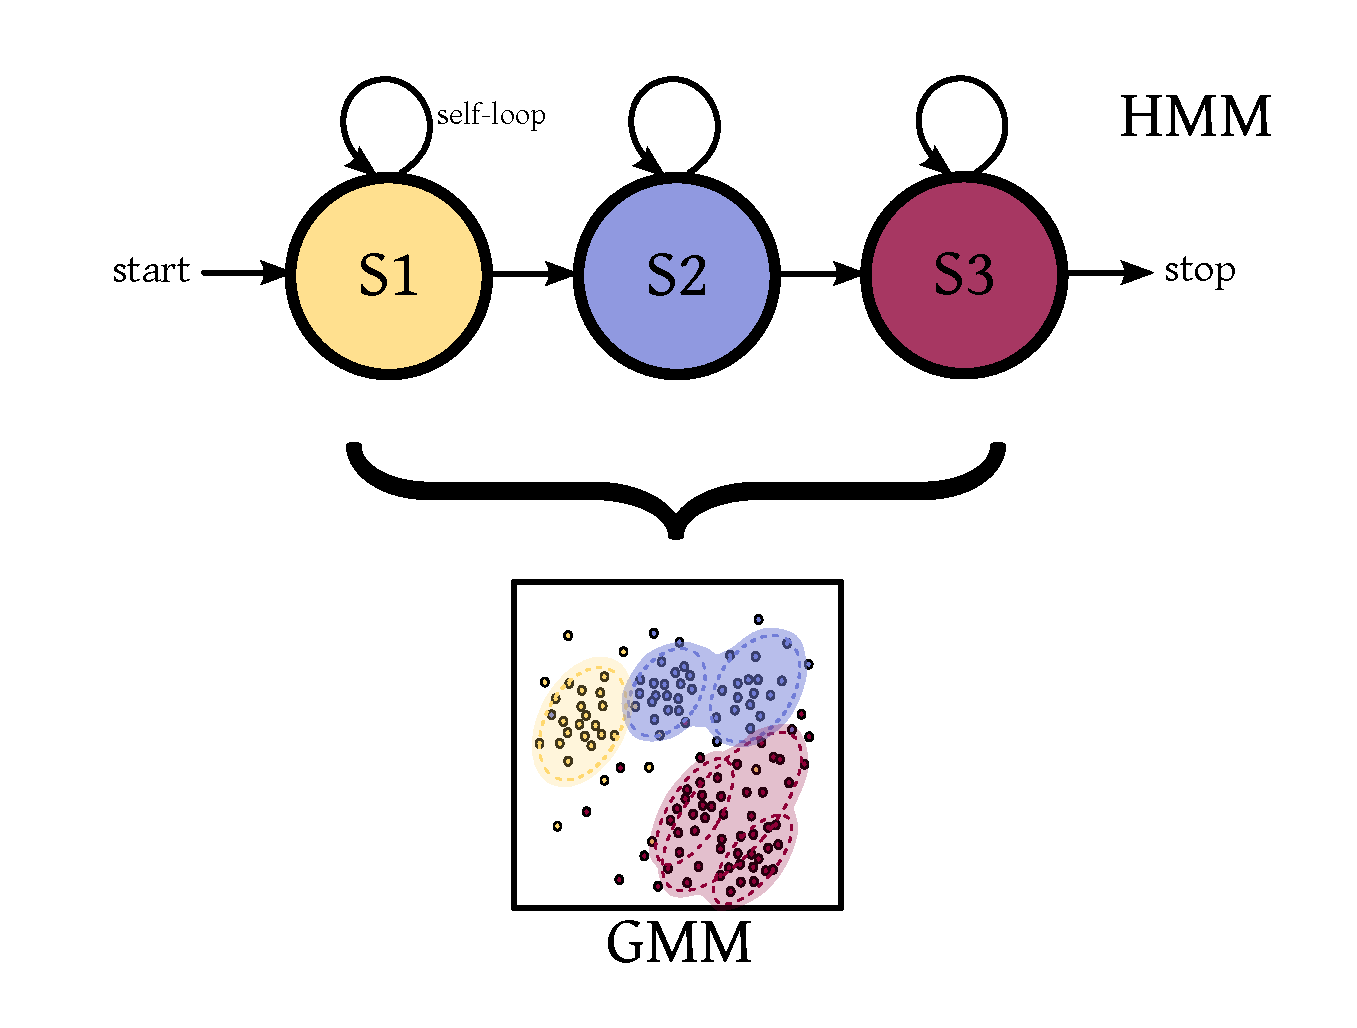
\includegraphics[width=0.6\linewidth]{chapter03/hmm_3state.pdf}
\caption{\textit{Left-to-right 3-state phoneme HMM with simplified 2-dimensional GMM (one per state). Start and stop states connect the phoneme with the previous and next phoneme, respectively.}}
\label{fig:hmm_3state}
\end{figure}

In sum, each phoneme is modelled by a left-to-right 3-state HMM. But what exactly is a state? Our acoustic models are HMM-GMMs, where GMM stands for Gaussian Mixture Models. For each phoneme our 48-dimensional feature vectors define a 48-dimensional space where GMM for the three states are embedded. During training, the acoustic model will have placed individual acoustic frames on this space, based on the values of their feature vector. In other words, acoustic frames from each phoneme portion will occupy a certain part of this space. For each state, we can parametrically define the space covered using mixtures of Gaussian distributions (the aforementioned GMMs). Indeed, GMMs are universal approximators of densities when given enough components. To do this, the model will have fitted a number of diagonal Gaussian distributions to approximate the distribution of datapoints corresponding to each phoneme state. The number of Gaussians allocated to each phoneme state depends on the total number of Gaussians made available to the model, and the complexity of the distribution of the frames in the space. Once that the GMMs are defined, the AM is able to tell us, for any new frame, the likelihood that the frame originated from each GMM (i.e., phoneme state).  \\     

\subsubsection{Why not triphones?}
If the reader is already familiar with ASR systems, they may expect us to go a step further and no longer treat phonemes as units for the HMMs (i.e., monophone acoustic models) but, instead, use context-dependent triphones. In this latter representation, an independent three-state HMM is built for each phoneme within a phonemic context. With some simplifications, this equates to no longer having an HMM for the phoneme \textipa{/p/}, but having all context-dependent versions of this phoneme as individual HMMs (e.g., the triphone \textipa{/p$_{a\_i}$/}, which is the phone \textipa{/p/} when preceded by \textipa{/a/} and followed by \textipa{/i/}).
Traditionally, triphone-based HMM-based ASR systems perform better than monophone systems. However, these more complex models are inappropriate for our experiments. Recall that we aim to use these speech recognition systems as models of nonnative speech perception, using tasks analogous to paradigms used in psycholinguistic experiments (namely, identification/forced-choice tasks). Importantly, we are focusing on modelling perceptual vowel epenthesis. This situation excludes the use of triphones because, by definition, our ASR systems will have to decode speech that does not follow native phonotactics. Decoding such stimuli implies the existence of triphones corresponding to the input, yet the model will have never encountered such triphones in the training data. While this situation might seem analogous to what listeners may experience, one must consider the fact that the ASR system \textit{will attempt to account for said triphones} during decoding in spite of the lack of data. Importantly, poorly estimated, phony triphones (e.g., \textipa{/h$_{a\_p}$/}, when decoding \textipa{/ahpa/}) will be put up against well-estimated triphones (e.g., \textipa{/h$_{a\_a}$/}) during the forced-choice tasks. The well-estimated triphones might simply be preferred as transcriptions over poorly-estimated ones for this reason alone, irrespective of the actual acoustic match between the stimuli and phoneme models.
In order to increase the performance of monophone models at phonetic labelling tasks such as ours, it is possible to increase the number of total Gaussians available to the model \cite{saraclar2001}. 

\subsection{Lexicon \& language models} \label{hmm_lm}
As shown in Figure \ref{fig:hmm_architecture}, the acoustic model is combined with two other components in order to decode speech: the Lexicon and the Language Model (LM).

The lexicon is, put simply, a pronunciation dictionary. It links the acoustic model (i.e., phoneme-level HMMs) with the language model, which is at the word level. For each word, we indicate in the dictionary the sequence of phonemes that constitute it. It is also possible to account for multiple pronunciations of a word due to dialectal differences (e.g., ``tomato'' pronounced as \textipa{/t@mA:t@U/} or \textipa{/t@meIRoU/}), phonological phenomena (e.g., homorganic assimilation: ``handbag'' \textipa{/h\ae ndb@g/} $\rightarrow$ \textipa{/h\ae mb@g/}), or supresegmental information (e.g., stress contrasts: ``record'' \textipa{/'rekord/} (noun) vs. \textipa{/re'kord/} (verb)).

At the word level, the language model specifies $P(W)$, the probability of occurrence of word sequence $W$. For this we use \textit{n}-grams: we approximate the probability of a sequence
\begin{equation}
P(W) = P(w_{1})P(w_2|w_1)P(w_3 | w_1, w_2)...P(w_L | w_1, w_2, ..., w_L)
\end{equation}
by using the product of the probability of the component words, each conditioned on the \textit{n-1} words preceding it. For instance, if $n = 2$, we obtain a bigram model, where the LM specifies the probability of a word depending on a single preceding word. The probability of the word sequence $W$ can then be approximated as:    
\begin{equation}
P(W) \approx P(w_{1})P(w_2|w_1)P(w_3 | w_2)...P(w_L | w_{L-1})
\end{equation}

In our case, these probabilities are obtained from word counts in the training corpus as follows:
\begin{equation}
P(w_i | w_j) \approx \frac{c(w_i, w_j)}{c(w_i)}
\end{equation}
where $c(w_i, w_j)$ is the number of observations of $w_i$ followed by $w_j$, and $c(w_i)$ is the total number of occurrences of $w_i$.
Since not all word combinations are bound to appear in the training corpus, smoothing is performed; null probabilities are given a small probability of appearing. 

Additionally to the bigram word LM, we computed a unigram phone LM in order to evaluate our models' ability to do phonetic decoding. In this case, the lexicon is identical to the phoneme inventory and the LM consists of phoneme counts.  

\subsection{Decoding}
When decoding speech, the ASR system builds a graph containing candidate word sequences that can serve as transcription for the audio input, based on the acoustic model, the lexicon, and the language model. In order to keep the problem computationally tractable, only the most likely transcription hypotheses are kept; this is known as pruning.

The output of the decoding step is not a single transcription but what is called a lattice. In this graphical representation only the most probable transcriptions are included, with weighted paths connecting words (a minimalistic example without weights can be seen in Figure \ref{fig:hmm_architecture}). The weight of each path is determined by the product of the acoustic and language model scores (derived from $P(X|w)$ and $P(W)$, respectively). The final score for each possible transcription is obtained by summing all the weights of the path that need to be crossed to reach the sequence of words in the transcription (``I love my cute dog'', in the example in Figure \ref{fig:hmm_architecture}). Having access to lattices means that we are not only able to derive the most probable transcription; we can extract the \textit{n}-best transcriptions, each with its corresponding alignment, and the total acoustic and language model scores.   

\subsection{Scoring: Assessing native performance}

\begin{figure}[htb]
\centering
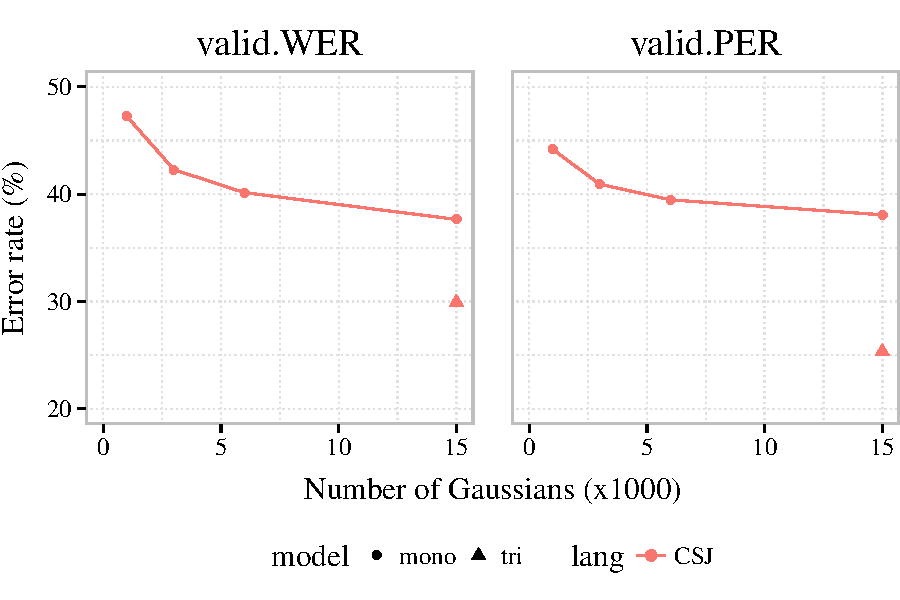
\includegraphics[trim={0 0 0 0}, clip, width=0.8\linewidth]{chapter03/ch3_misc_plotting/figures/plot_hmm_evaluations.pdf}
\caption{\textit{Changes in word error rate (\%WER) and phone error rate (\%PER) following variation of the number of total Gaussians allocated to monophone acoustic models (circles). The error rates obtained with a triphone model with $15,000$ Gaussians are included as comparison (triangles). Scores correspond to decoding performed on the validation set (i.e., unseen speakers for the CSJ and KCSS; already seen speakers for the WSJ).}}
\label{fig:hmm_gaussians}
\end{figure}


We tested the decoding performance on the validation set of AMs with total number of Gaussians going from $1,000$ to $15,000$. These values are used as default total number of Gaussians when training, respectively, monophone and triphone models in Kaldi (without speaker adaptation).
In order to do so, we used the language models described in section \ref{hmm_lm}, namely a word bigram LM and a phone unigram LM, which were used to obtain word error rates (\%WER) and phone error rates (\%PER), respectively. Note that while we provide word bigram WER\% as a reference value to compare with existing speech recognition models\footnote{As a reference, in 2015 some state-of-the-art speaker adapted HMM-GMM systems trained on 82 hours of the WSJ achieved $6.26\%$ WER \cite{panayotov2015} and $5.39\%$ WER \cite{chan2015} on the WSJ eval'92 dataset. Contemporary deep neural network-based systems achieved $3.47\%$ WER on the same dataset \cite{chan2015}.}, our main focus is on PER\%. Indeed, we will use our models in paradigms involving phonetic decoding of non-native nonwords; the phone unigram PER\% evaluation gives us an insight into how well our ASR systems can do phonetic decoding on native (non)words. 

As seen in Figure \ref{fig:hmm_gaussians}, we find that the performance of our models increased (i.e., error rates decreased) when increasing the number of total Gaussians from the Kaldi default of $1,000$ to $15,000$, which would average to approximately $125$ Gaussians per state for a language with an inventory of 35 phonemes\footnote{Phoneme counts: CSJ: 37, KCSS: 36, WSJ: 39}.   
Therefore, the acoustic models with the highest amount of Gaussians (i.e., $15,000$) give the best performance for monophone models, both at the lexical (\%WER) and phonetic (\%PER) levels of decoding.
We did not pursue increasing the number of Gaussians even further, as performance gain was reaching an asymptote at this point and adding more Gaussians would have increased the computational demands for each experiment. Additionally, we expect that adding ``too many'' Gaussians might have lead to overfitting of the models to the training set.
As expected, triphone models performed better than monophone models at phonetic decoding (\%PER), in spite of having the same amount of total Gaussians than our best monophone models (CSJ: $37.96\%$ monophone \textit{vs.} $25.33\%$ triphone; KCSS: $50.70\%$ monophone \textit{vs.} $38.42\%$ triphone). Later in this chapter we will discuss how it might be possible to increase acoustic model performance in future work, without having recourse to triphone HMMs, which as explained previously are not appropriate for our experiments.  

Concerning the test set (i.e., $15\%$ of the corpora), we find \%WER comparable to those obtained for the validation set (CSJ: $37.48\%$ on test, $37.64\%$ on validation; KCSS: $73.35\%$ on test, $74.03\%$ on validation), and similarly for \%PER (CSJ: $37.96\%$ on test, $38.07\%$ on validation; KCSS: $50.70\%$ on test and validation).
Since the validation and test sets contain utterances from the same speakers, this information does not allow us to evaluate our models' sensitivity when decoding data from speakers not used in the training data (recall that none of our models have any speaker adaptation; only CMVN is applied when processing the features). However, the fact that validation and test set scores are similar indicates that, while rudimentary, our acoustic models give stable performances when confronted with datasets with structurally different lexical exemplars and acoustically different phonetic exemplars.   

{\color{red}[TODO]: Add WSJ}
%> d.eval
%   corpus model totgauss   set   WER   PER
%1     CSJ  mono        1 valid 47.24 44.16
% 2     CSJ  mono        3 valid 42.28 40.92
% 3     CSJ  mono        6 valid 40.14 39.47
% 4     CSJ  mono       15 valid 37.64 38.07
% 5     CSJ   tri       15 valid 29.94 25.33
% 6     CSJ  mono       15  test 37.48 37.96

% 7    KCSS  mono        1 valid 81.39 56.23
% 8    KCSS  mono        3 valid 77.20 53.05
% 9    KCSS  mono        6 valid 75.59 51.66
% 10   KCSS  mono       15 valid 74.03 50.70
% 11   KCSS   tri       15 valid 65.48 38.42
% 12   KCSS  mono       15  test 73.35 50.70

% 13    WSJ  mono        1 valid 18.54    NA
% 14    WSJ  mono        3 valid 14.55    NA
% 15    WSJ  mono        6 valid 12.81    NA
% 16    WSJ  mono       15 valid 11.26    NA
% 17    WSJ   tri       15 valid  8.48    NA
% 18    WSJ  mono       15  test 11.50    NA

%%%%%%%%%%%% 
% Parlato2 %
%%%%%%%%%%%%
%\section{{\color{red}Parlato-hmm}} \label{3-parlato-hmm} [Merged into SurfPhono]

%%%%%%%%%%%%%
% SurfPhono %
%%%%%%%%%%%%%
\newpage
\section{{\color{red}Investigating surface phonotactics}} \label{3-surfphono}

\small{\textit{{\color{red}ADD ACKNOWLEDGEMENTS THOMAS + EMMANUEL.\\}}}

\subsection{Introduction}

{\color{red}[TODO]}
%%% Background

%%% Goal
% Test acoustic model (null)
% Compare with more informative LMs

%%% Plan

\subsection{Experiment 1: {\color{red}m-/ahpa/}}
\subsubsection{Methods}
\paragraph{Stimuli}
We used the same stimuli as in section \ref{2-ahpa}. As a reminder, we recorded 3 speakers producing disyllabic $V_{1}C_{1}C_{2}V_{1}$ and trisyllabic $V_{1}C_{1}V_{2}C_{2}V_{1}$, with $V_{1}$ a flanking vowel in the set \textipa{/a, e, i, o, u/}, $C_{1}$ \textipa{/h/} or /k/, and $C_{2}$ a fixed consonant, /p/ (e.g, \textipa{/ahpa/}, \textipa{/ahapa/}). By cross-splicing the disyllabic natural control items (e.g., \textipa{/ahpa/}), we obtained disyllabic spliced control items (e.g., \texorpdfstring{\textipa{/ah\textsubscript{a}pa/}}{}), disyllabic spliced test stimuli (e.g., \texorpdfstring{\textipa{/ah\textsubscript{u}pa/}}{}), and trisyllabic spliced fillers (e.g., {\textipa{/ahapa/}), where subscripts indicate the identity of the vowels flanking the clusters in the original recording. Therefore, within each speaker, all stimuli of the same structure (in our example, \textipa{/ah($V$)pa/} items) have acoustically identical flanking vowels.
  
\paragraph{Language models}
In order for the decoding task to be analogous to the behavioural experiment described in section \ref{2-ahpa}, trial-specific language models were constructed, as shown in Figure \ref{fig:m-ahpa_G}. Thus, when decoding a $V_{1}C_{1}(V_{2})C_{2}V_{1}$ stimulus, the perception model was only given the possibility to transcribe it as $V_{1}C_{1}(V_{2})(SIL)C_{2}V_{1}$, where phones between parentheses are optional, $V_{2}$ was from the set of vowels \textipa{/a, e, i, o, u/}, and $SIL$ is an optional silence. 

\begin{figure}[htb]
    \centering
    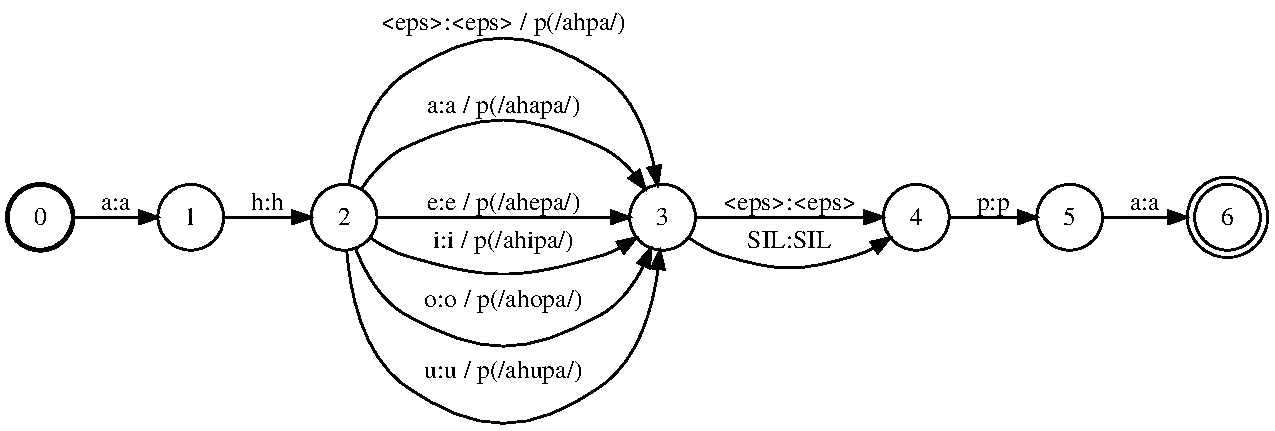
\includegraphics[width=0.8\linewidth]{chapter03/m-ahpa_Gfst.pdf}
    \caption{\textit{Constrained language model used to test the models (here: LM for \textipa{/ahpa/} trials). Nodes in the graph represent states, weighted edges represent transitions between states (here: phonemes). When relevant, weighted edges are labeled with the probability to choose that edge when decoding, which affects the final language model score of each possible path. When no weights are shown (e.g., between states 3 and 4), there is no preference between the paths concerned. The language model scores are combined with acoustic scores when decoding experimental items.}}
    \label{fig:m-ahpa_G}
\end{figure}

In this section, we investigate the type of phonotactic information that might be used by Japanese listeners when perceiving foreign speech that does not conform to native phonotactics. We test 5 types of language models (LM) when decoding our $V_{1}C_{1}(V_{2})C_{2}V_{1}$ items; these LMs differ only in the weights given to edges between nodes 2 and 3 in the graph shown in Figure \ref{fig:m-ahpa_G}. The weights were obtained by computing frequency counts from the portion of the CSJ used for training the acoustic model. Using the same acoustic model, we compared the following LMs {\color{red}[TODO] Add formulae as annex}: 

\begin{enumerate}
    \item A null LM, which implies that listeners base their decoding of consonant clusters on phonetic match alone, without using information on phonotactics.
    \item A phone-unigram LM, which implies that listeners do not take neighbouring phonemes into consideration when decoding the consonant clusters; only the frequency of the vowel $V_{2}$ to be epenthesized (compared to that of $C_{2}$) is taken into account when choosing epenthetic vowel quality.
    \item An online phone-bigram language model, which implies that listeners decode the clusters as they hear them (i.e., decoding is done from the start of the item), and the choice of (no) vowel is conditioned on the presence of $C_{1}$. Therefore, the choice of epenthetic vowel is modulated by $C_{1}V_{2}$ and $C_{1}C_{2}$ diphone frequencies. 
    \item A retro phone-bigram language model, which implies that listeners decode the clusters based on the most recent information (i.e., decoding is done from the end of the item), and the choice of (no) vowel is conditioned on the presence of $C_{2}$. Thus, the choice of epenthetic vowel is modulated by $V_{ep}C_{2}$ and $C_{1}C_{2}$ diphone frequencies.
    \item A batch phone-bigram language model, which implies that listeners decode the item considering the entire structure, taking into consideration the probability of having a vowel $V_{2}$ given the presence of $C_{1}$ and $C_{2}$. Here the choice of epenthetic vowel is modulated by the product of $C_{1}V_{2}$ and $V_{2}C_{2}$ (or by $C_{1}C_{2}$) diphone frequencies.  
\end{enumerate}
    
\paragraph{Identification task simulation}
\begin{figure}[htb]
  \centering
  \begin{overpic}[trim={0 1cm 0 1.5cm},clip, width=0.7\linewidth]{chapter03/m-ahpa_praat_ah0apa.pdf}\end{overpic}
  \caption{\textit{Example of how the ASR system decodes the item \textipa{/ah$_{a}$pa/}, using the null version of the language model in Figure \ref{fig:m-ahpa_G}. From top to bottom: original waveform, item name, aligned transcriptions given by the model (from the most probable to the least probable, with the corresponding posteriorgrams shown to their right side), and spectrogram with formant contours. SIL = silence.}}
  \label{fig:m-ahpa_align}
\end{figure}

After decoding the stimuli, we extracted from the resulting lattice each possible transcription of each item, and the corresponding acoustic and language model scores. An example of how the ASR system decodes the experimental stimuli can be seen in Figure \ref{fig:m-ahpa_align}. From the (scaled) acoustic and language model scores we derived the item posteriorgrams, which indicate how probable a given transcription was given the audio input. We used these probabilities as proxies of the probability that a listener might exploit when performing reverse inference during speech perception, and therefore, the probabilities used when responding in an identification task. 

As such, for each item, we obtained a six-dimensional vector $ident_{model} = [p_{none}, p_{a}, p_{e}, p_{i}, p_{o}, p_{u}]$, containing a discrete probability distribution, with a probability mass function linking the identification task options `none', `a', `e', `i', `o', `u', to their respective probabilities (i.e., posteriorgrams).
We can define the human equivalent $ident_{human} = [p_{none}, p_{a}, p_{e}, p_{i}, p_{o}, p_{u}]$, which contains the percentage of responses for each item, after aggregating all participant responses. 

\subsubsection{Quantitative analysis}
In order to perform a global evaluation of the similarity between the behavioural responses and the responses obtained with the five LMs described above, we computed the Pearson's product-moment correlation coefficient between the human and model posteriorgrams. The model with the highest correlation to the human data was the \textsc{null} LM ($r = 0.76$), followed by the \textsc{unigram}, \textsc{bigram online}, and \textsc{bigram retro} LMs ($r = 0.65$), and lastly, the \textsc{bigram batch} LM ($r = 0.62$). Numerically, the \textsc{null} LM better approximated the human data.

In order to assess if the correlation differences between the \textsc{null} LM and other LMs were significant, we computed these differences and their corresponding 95\% confidence intervals (CIs), using bootstrapping with 1000 samples\footnote{Sampling was done by item.}. As can be seen in Table \ref{tab:m-ahpa-cor_diff}, the correlation between the human data and the output of the \textsc{null} LM was significantly higher than those of other LMs.

% latex table generated in R 3.3.3 by xtable 1.8-2 package
% Mon Jul  2 21:36:40 2018
\begin{table}[htb!]
\centering
\caption{\textit{Difference in correlation with human data between the null LM and other LMs. The lower and upper bounds of the 95\% confidence intervals are given between brackets. Positive values indicate higher correlation between human data and null model output than between human data and other LM output.}}
  \label{tab:m-ahpa-cor_diff}
\vspace{0.25cm}
\begin{tabular}{lccc}
  \toprule
 & Correlations & Difference & Significant? \\  \midrule
null vs. unigram & $0.76 - 0.65$ & $0.10$ $[0.07, 0.14]$ & Yes \\ 
  null vs. bigram online & $0.76 - 0.65$ & $0.11$ $[0.08, 0.14]$ & Yes \\ 
  null vs. bigram retro & $0.76 - 0.65$ & $0.10$ $[0.07, 0.13]$ & Yes \\ 
  null vs. bigram batch & $0.76 - 0.62$ & $0.13$ $[0.10, 0.17]$ & Yes \\ \bottomrule 
\end{tabular}
\end{table}

Contrary to the null and unigram LMs, the bigram models were subject to an arbitrarily set smoothing parameter, which determined the probability of choosing a sequence of phonemes that had never been observed in the training data. We set this smoothing parameter to $10^{-8}$, which is a strict value, as it is relatively close to zero. This was done in order to evaluate whether the acoustic match could rescue decoding options which are not supported by the language's phonotactics. In order to evaluate the similarity between models' outputs and human data without the influence of the value of the smoothing parameter, we computed the correlation between the human data and models' posteriorgrams after excluding the posteriorgrams for ``none'' responses and re-normalising the remaining posteriorgrams. As such, we are focusing on the correlation related to epenthetic vowel quality.
Here, the highest correlation still corresponded to the \textsc{null} LM ($r = 0.77$), followed by the \textsc{bigram retro} ($r = 0.74$), the \textsc{bigram online} ($r = 0.73$), and finally the \textsc{unigram} and the \textsc{bigram batch} LMs ($r = 0.71$). 
As shown in Table \ref{tab:m-ahpa-cor_diff-nonone}, while the difference between the correlations diminished relative to what is shown in Table \ref{tab:m-ahpa-cor_diff}, the CIs still did not overlap with zero, meaning that the correlation between the human data and the output of the \textsc{null} LM was significantly higher than those of other LMs.  

% latex table generated in R 3.3.3 by xtable 1.8-2 package
% Tue Jul  3 03:37:50 2018
\begin{table}[htb!]
\centering
\caption{\textit{Difference in correlation with human data between the null LM and other LMs, after removing the ``none'' responses. The lower and upper bounds of the 95\% confidence intervals are given between brackets. Positive values indicate higher correlation between human data and null model output than between human data and other LM output.}}
\label{tab:m-ahpa-cor_diff-nonone}
\vspace{0.25cm}
\begin{tabular}{lccc}
   \toprule
  & Correlations & Difference & Significant? \\  \midrule
  null vs. unigram & $0.77 - 0.71$ & $0.05$ $[0.03, 0.08]$ & Yes  \\  
  null vs. bigram online & $0.77 - 0.73$ & $0.04$ $[0.02, 0.06]$ & Yes \\   
  null vs. bigram retro & $0.77 - 0.74$ & $0.02$ $[0.01, 0.04]$ & Yes \\ 
  null vs. bigram batch & $0.77 - 0.71$ & $0.06$ $[0.03, 0.08]$ & Yes \\ \bottomrule 
\end{tabular}
\end{table}

\subsubsection{Qualitative analyses}

\paragraph{Identification accuracy}
Using the set of filler items such as \textipa{/ahapa/} and \textipa{/okipo/} (i.e., spliced items with a full vowel between $C_1$ and $C_2$), we can assess identification accuracy relative to our item labels. Indeed, recall that while our phonetically-trained speakers were instructed to read items following ``standard'' IPA pronunciations, it is possible for our human participants to not perceive the intended vowel categories due to adaptation processes (e.g., misperceiving \textipa{/u/}, which is not realised as \textipa{[u]} but as \textipa{[W]} in Japanese), and/or due to speaker idiosyncrasies.

\begin{figure}[htb]
\centering
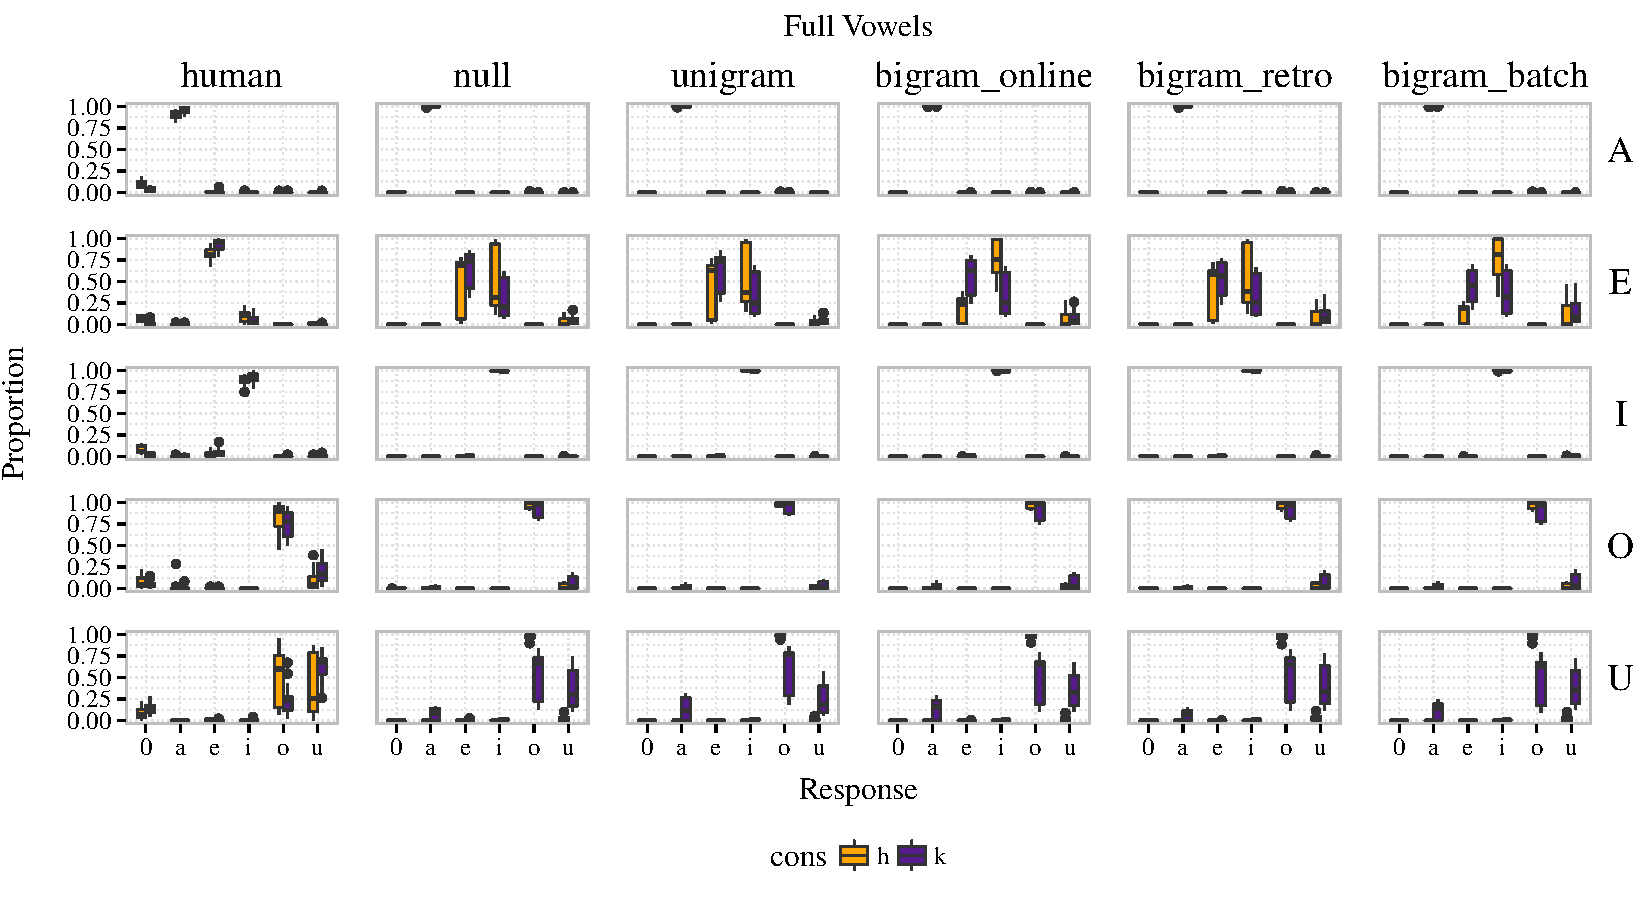
\includegraphics[width=1\linewidth]{chapter03/m-ahpa_figures.pdf}
\caption{\textit{{\color{red}TODO}}}
\label{fig:m-ahpa_fV_acc}
\end{figure}

Overall, human participants identified the correct intended vowel category in $79.5\%$ of the trials. As can be seen in Figure \ref{fig:m-ahpa_fV_acc}, this was mostly due to confusions between the intended \textipa{/o/} and \textipa{/u/} categories, with most errors being \textipa{/u/} being identified as \textipa{/o/}.
Consistent with our correlation analyses, the \textsc{null} LM gave the highest accuracy out of all models (accuracy: $74\%$), followed by the \textsc{bigram retro} (accuracy: $72.6\%$), the \textsc{unigram} (accuracy: $72.5\%$), the \textsc{bigram online} (accuracy: $72.6\%$), and finally the \textsc{bigram batch} LM (accuracy: $68.7\%$). 
As seen in Figure \ref{fig:m-ahpa_fV_acc}, like human participants, the models showed difficulty categorising \textipa{/u/} items as such; in particular, these were almost always classified as exemplars of \textipa{/o/} when $C_2 = \textipa{/h/}$. However, unlike human participants, models misperceived \textipa{/e/} as \textipa{/i/}. This misperception appears to be worse for the \textsc{bigram online} and \textsc{bigram batch} language models.
In sum, while the accuracy rates for the models were close to that of humans, we saw that the models showed not only quantitative but also qualitative differences in their identification of non-native full vowels, in comparison with human participants. Below we continue our qualitative analyses on what was determined to be the best model according to the correlation analyses and the filler item accuracy, namely the ASR system with a \textsc{null} LM.  

\paragraph{Control items}
Human participants experienced vowel epenthesis in $56\%$ (\textipa{/hp/}: $52\%$; \textipa{/kp/}: $61\%$)\footnote{Note that since posteriorgrams are computed by weighting items from all three speakers are equally, values reported in this section might differ slightly from those in section \ref{2-ahpa}. Indeed, due to how data was cleaned in section \ref{2-ahpa}, some trials were removed and the number of trials per item per speaker might have differed in some cases. In order to ensure that human and model data are comparable, we re-do statistical analyses of human data when necessary and report the resulting coefficients.} of control items in which the flanking vowel and coarticulation are of the same quality. The \textsc{null LM} gave an output of $68\%$ epenthesis, with $72\%$ and $65\%$ epenthesis for \textipa{/hp/} and \textipa{/kp/}, respectively. As such, the model gave a higher percentage of epenthesis for \textipa{/hp/} clusters compared to \textipa{/kp/}clusters, while the opposite was true for humans.

Now we focus on epenthetic vowel quality, meaning that we perform analyses after removing ``none'' responses and re-normalising posteriorgrams. We find that, like humans (\textipa{/hp/}: $44\%$; \textipa{/kp/}: $87\%$; total: $66\%$), the model gave lower percentages of default \textipa{/u/}-epenthesis for \textipa{/hp/} ($47\%$) than \textipa{/kp/} ($65\%$) clusters (total: $56\%$). However, this difference is not as marked as it is for humans. Recall that in section \ref{2-ahpa} we found that humans experiences significantly more default \textipa{/u/}-epenthesis for \textipa{/kp/} clusters, while experiencing significantly more vowel copy epenthesis for \textipa{/hp/} clusters. These patterns of responses mirrored loanword data. Do we find these effects in the output of our model? 

We first examined possible effects of consonant cluster on default \textipa{/u/}-epenthesis by using the R statistical software \cite{R-base}, using Markov chain Monte Carlo generalised linear mixed-models \cite{R-MCMCglmm, R-coda}. These Bayesian models sample coefficients from the posterior probability distribution conditioned on the data and given priors. We used priors that are standard for linear models. Model convergence was assessed by visual inspection of trace plots and the Gelman–Rubin convergence diagnostic \cite{gelman1992}, using eight chains with different initialisations. Effects were considered statistically significant if the 95\% highest posterior density (HPD) interval estimated for the coefficient of interest did not include zero. We report both the posterior mode and the 95\% HPD interval.  

The left panel of Figure \ref{fig:m-ahpa_ctrl} shows the posteriograms of \textipa{/u/}-epenthesis for humans and all models. For the ASR system with the null LM, we assessed the variation of the continuous response variable ``u'' response \textsc{Posteriorgram} that was caused by the fixed effect \textsc{Consonant} cluster (\textipa{/kp/} \textit{vs.} \textipa{/hp/}; contrast coded with deviance coding).
We initially included random intercepts for \textsc{Speaker} and \textsc{Item}, as well as a random slope for \textsc{Speaker} on \textsc{Consonant}. However, these were removed as their addition caused the models to be singular (estimated null variances), with consequently poor trace plots.
We found the main effect of \textsc{Consonant} to be significant (mode: $-0.19$, HPD: $[-0.29,-0.07]$), meaning that as for humans (mode: $-0.42$, HPD: $[-0.61,-0.26]$), the model gave significantly more \textipa{/u/}-epenthesis for \textipa{/hp/}- than \textipa{/kp/}-clusters. However, as evidenced by the statistical model coefficients, the magnitude of the effect is larger for humans than for the model.  

\begin{figure}[htb]
\centering
\includegraphics[page=8, width=1\linewidth]{chapter03/m-ahpa_figures.pdf}
\caption{\textit{{\color{red}TODO}}}
\label{fig:m-ahpa_ctrl}
\end{figure}

Turning to vowel copy epenthesis in control items for which the flanking vowel was not \textipa{/u/}, we used the same statistical models but with copy vowel \textsc{Posteriorgram} as the continuous response variable. For instance, for the item \textipa{/ek$_{e}$pe/}, this was the posteriorgram for the ``e'' response. The distribution of posteriorgrams for humans and all models is shown in the right panel of Figure \ref{fig:m-ahpa_ctrl}.
While there was a trend in the same direction for the null LM, namely higher percentages of vowel copy for \textipa{/hp/}- than \textipa{/kp/}-clusters, we did not find a significant main effect of \textsc{Consonant} for the model (mode: $0.11$, HPD: $[-0.02, 0.24]$) as we did for humans (mode: $0.39$, HPD: $[0.20, 0.58]$). 

\paragraph{Test items}
{\color{red}[TODO]}

As shown in Figure \ref{fig:m-ahpa_test_coll}, reponses that were represented the most in the null model posteriorgrams were ``none'' (\%), ``i'' (\%), and ``u'' (\%). These were also the responses that human participants gave the most (``none'' (\%), ``i'' (\%), and ``u'' (\%)).

\begin{figure}[htb!]
\centering
\includegraphics[page=5, width=0.75\linewidth]{chapter03/m-ahpa_figures.pdf}
\caption{\textit{{\color{red}TODO}}}
\label{fig:m-ahpa_test_coll}
\end{figure}

\begin{figure}[htb!]
\centering
\includegraphics[page=4, width=1\linewidth]{chapter03/m-ahpa_figures.pdf}
\caption{\textit{{\color{red}TODO}}}
\label{fig:m-ahpa_test}
\end{figure}


\subsection{Experiment 2: {\color{red}Parlato-lms}}
\subsubsection{Methods}
\paragraph{Stimuli}
We used the same stimuli as in sections \ref{2-parlato} and \ref{2-parlato-dur}. As a reminder, a native French speaker recorded 54 items with the structure $V_{1}C_{1}C_{2}V_{2}$, with $V_{1}$ and $V_{2}$ vowels from the set \{/a/, /i/, /u/\}, and $C_{1}C_{2}$ a cluster from the set \{/bg/, /bn/, /db/, /dg/, /gb/, /gn/\} (e.g. /abgi/).

\paragraph{Language models}

In order for the decoding task to be analogous to the behavioural experiment described in section \ref{2-parlato_per}, trial-specific language models were constructed, as shown in Figure \ref{fig:parlato_G}. Thus, when decoding a $V_{1}C_{1}C_{2}V_{2}$ stimulus, the perception model was only given the possibility to transcribe it as $V_{1}C_{1}(V_{ep})(SIL)C_{2}V_{2}$, where phones between parentheses are optional and $V_{ep}$ was from the set of vowels \textipa{/a, e, i, o, u/}, and $SIL$ is an optional silence. Concerning the weights between states 2 and 3, we created language models in a way analogous to the LMs in Experiment 1, adapted to the $V_{1}C_{1}C_{2}V_{2}$ items used in this experiment.

\begin{figure}[htb]
\centering
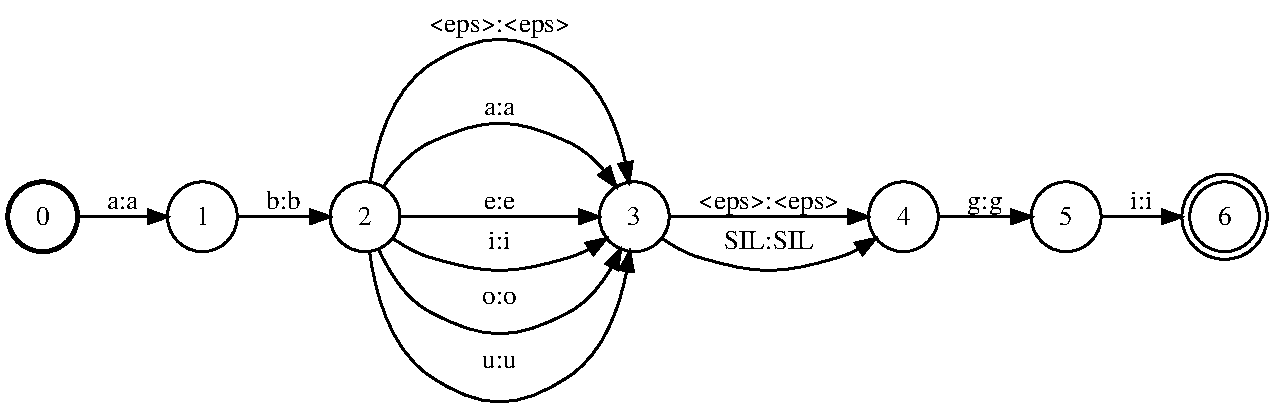
\includegraphics[width=0.8\linewidth]{chapter03/parlato_hmm_Gfst.pdf}
\caption{Constrained language model used to test the models (here: LM for decoding \textipa{/agni/}). Nodes in the graph represent states, weighted edges represent transitions between states (here: phonemes). When relevant, weighted edges are labeled with the probability to choose that edge when decoding, which affects the final language model score of each possible path. When no weights are shown (e.g., between states 3 and 4), there is no preference between the paths concerned. The language model scores are combined with acoustic scores when decoding experimental items.
}
\label{fig:parlato_G}
\end{figure}

\paragraph{Identification task simulation}
We used the same procedure as in Experiment 1. An example of how the ASR system decodes the experimental stimuli can be seen in Figure \ref{fig:parl_hmm_align}. 

\begin{figure}[htb!]
  \centering
  \begin{overpic}[trim={0 2.5cm 0 1.5cm},clip, width=0.7\linewidth]{chapter03/parlato-hmm_praat_agni.pdf}\end{overpic}
  \caption{\textit{Example of how the ASR system decodes the item \textipa{/agni/}, using the null version of the language model in Figure \ref{fig:parlato_G}. From top to bottom: original waveform, item name, aligned transcriptions given by the model (from the most probable to the least probable, with the corresponding posteriorgrams shown to their right side), and spectrogram with formant contours. SIL = silence.}}
  \label{fig:parl_hmm_align}
\end{figure}

\subsubsection{Results: Quantitative analysis}
As in Experiment 1, we computed the Pearson's product-moment correlation coefficient between the human and model posteriorgrams in order to assess a global measure ressemblance between models' outputs and the human data from section \ref{2-parlato_per}. The model with the highest correlation to the human data was the \textsc{bigram retro} LM ($r = 0.43$), followed by the \textsc{null} ($r = 0.40$), the \textsc{unigram} ($r = 0.30$), the \textsc{bigram online} ($r = 0.23$) and lastly, the \textsc{bigram batch} LM ($r = 0.19$). Numerically, the \textsc{bigram retro} LM better approximated the human data.

In order to assess if the correlation differences between the \textsc{null} LM and other LMs were significant, we computed these differences and their corresponding 95\% confidence intervals (CIs), using bootstrapping with 1000 samples. As can be seen in Table \ref{tab:parlato_lms-cor_diff}, the correlation between the human data and the output of the \textsc{null} LM was significantly higher than those of the \textsc{unigram}, \textsc{bigram online} and \textsc{bigram batch}. While the correlation to the human data for \textsc{bigram retro} LM was numerically higher than for the \textsc{null} LM, we did not find evidence of a significant difference between the two as the CI of their difference overlaps zero.

% latex table generated in R 3.3.3 by xtable 1.8-2 package
% Tue Jul  3 03:53:37 2018
\begin{table}[ht]
\centering
\caption{\textit{Difference in correlation with human data between the null LM and other LMs. The lower and upper bounds of the 95\% confidence intervals are given between brackets. Positive values indicate higher correlation between human data and null model output than between human data and other LM output.}}
\label{tab:parlato_lms-cor_diff}
\vspace{0.25cm}
\begin{tabular}{lccc}
   \toprule
  & Correlations & Difference & Significant? \\  \midrule
null vs. unigram & $0.40 - 0.30$ & $0.11$ $[0.03, 0.18]$ &  Yes \\ 
null vs. bigram online  & $0.40 - 0.23$ & $0.18$ $[0.03, 0.31]$ &  Yes \\ 
null vs. bigram retro & $0.40 - 0.43$ & $-0.03$ $[-0.13, 0.08]$ &  No \\ 
null vs. bigram batch & $0.40 - 0.19$ & $0.21$ $[0.06, 0.35]$ & Yes \\  \bottomrule 
\end{tabular}
\end{table}

Similarly to how we did in Experiment 1, we evaluated the similarity between models' outputs and human data without focusing on percentage of vowel epenthesis. For this we computed the correlation between the human data and models' posteriorgrams after excluding the posteriorgrams for ``none'' responses and re-normalising the remaining posteriorgrams. Recall that, as a consequence, we are focusing on the correlation related to epenthetic vowel quality. The highest correlation corresponded to the \textsc{null} LM ($r = 0.53$), followed by \textsc{bigram retro} ($r = 0.46$), \textsc{unigram} ($r = 0.33$), \textsc{bigram online} ($r = 0.21$), and \textsc{bigram batch} ($r = 0.17$). 
As can be seen in Figure \ref{tab:parlato_lms-cor_diff-nonone}, the correlation between the human data and the output of the \textsc{null} LM was significantly higher than those between the human data and other LMs. 

% latex table generated in R 3.3.3 by xtable 1.8-2 package
% Tue Jul  3 04:00:07 2018
\begin{table}[ht]
\centering
\caption{\textit{Difference in correlation with human data between the null LM and other LMs, after removing the ``none'' responses. The lower and upper bounds of the 95\% confidence intervals are given between brackets. Positive values indicate higher correlation between human data and null model output than between human data and other LM output.}}
\label{tab:parlato_lms-cor_diff-nonone}
\vspace{0.25cm}
\begin{tabular}{lccc}
   \toprule
  & Correlations & Difference & Significant? \\  \midrule
null vs. unigram & $0.53 - 0.33$ & $0.21$ $[0.16, 0.26]$ & Yes  \\ 
null vs. bigram online   & $0.53 - 0.21$ & $0.33$ $[0.18, 0.46]$ & Yes \\ 
null vs. bigram retro    & $0.53 - 0.46$ & $0.08$ $[0.04, 0.12]$ & Yes \\ 
 null vs. bigram batch    & $0.53 - 0.17$ & $0.36$ $[0.21, 0.51]$ & Yes \\  \bottomrule 
\end{tabular}
\end{table}

\subsubsection{Results: Qualitative analysis}

\paragraph{Default vowel}

\begin{figure}[htb!]
    \centering
    \includegraphics[page=2, width=1\linewidth]{chapter03/parlato-lms_figs.pdf}
    \caption{\textit{Distribution of the proportion of responses given by human participants (leftmost panels) and posteriorgrams obtained when decoding with different language models. The box and whiskers plots display the distribution of posteriorgrams across experimental items, with boxplots separated according to the $C_{1}$ in the cluster and the responses (rows).}}
    \label{fig:parlato-lms}
  \end{figure}

{\color{red}Describe graph showing response patterns}

% 1     0         human 0.13071895
% 2     a         human 0.01416122
% 3     e         human 0.02505447
% 4     i         human 0.15250545
% 5     o         human 0.04684096
% 6     u         human 0.63071895
% 7     0          null 0.27663941
% 8     a          null 0.05414450
% 9     e          null 0.11487889
% 10    i          null 0.22482459
% 11    o          null 0.08025081
% 12    u          null 0.24926179

%In order to compare how well LMs compared at mimicking human behaviour, we computed the Euclidean distance between $ident_{LM}$ and $ident_{human}$ for each item, for each LM. Do models that integrate information about phoneme probabilities (i.e., \textsc{unigram} LM) or diphone probabilities (i.e., \textsc{bigram} LMs) show smaller \textsc{Eucl. distances} to human data than the \textsc{null} LM?

%The response variable of our statistical models was the \textsc{Eucl. distance} between $ident_{LM}$ and $ident_{human}$, as described above. We chose as fixed effect the \textsc{Language Model} (\textsc{LM}) used during decoding, considered as a categorical variable with \textsc{null} as the reference level. The variable was contrast coded with simple coding, meaning that non-reference levels were compared to the reference level, with the intercept corresponding to the grand mean (all levels). \textsc{$C_{1}$} was added as a random intercept.

%Statistical analyses were performed with the R statistical software \cite{R-base}, using Markov chain Monte Carlo generalised linear mixed-models \cite{R-MCMCglmm, R-coda}. These Bayesian models sample coefficients from the posterior probability distribution conditioned on the data and given priors. We used priors that are standard for linear models. Model convergence was assessed by visual inspection of trace plots and the Gelman–Rubin convergence diagnostic \cite{gelman1992}, using eight chains with different initialisations. Effects were considered statistically significant if the 95\% highest posterior density (HPD) interval estimated for the coefficient of interest did not include zero. We report both the posterior mode and the 95\% HPD interval.

%We found that, relative to the \textsc{null} LM, the \textsc{bigram online} (mode: $0.08$, HPD: $[0.02, 0.15]$) and the \textsc{bigram batch} (mode: $0.08$, HPD: $[0.02, 0.15]$) language models resulted in significantly higher Euclidean distances between the model responses and human responses. On the other hand, we did not find evidence of a difference between the \textsc{null} LM and the \textsc{unigram} (mode: $0.03$, HPD: $[-0.04, 0.10]$) or \textsc{bigram retro} (mode: $0.0$, HPD: $[-0.06, 0.07]$) language models.

%%\subsubsection{Overall similarity}
%\begin{figure}[H]
%  \centering
%   \begin{overpic}[trim={0 0 0 0.75cm}, clip, page=1, width=0.5\linewidth]{chapter03/parl_hmm_figs}\end{overpic}
%   \caption{\textit{Distribution of posteriorgrams obtained when decoding with a null language model. The box and whiskers plots display the distribution of posteriorgrams across experimental items.}}
%   \label{fig:parl_hmm_overall}
% \end{figure}
% Figure \ref{fig:parl_hmm_overall} shows the distribution of posteriorgrams for each response, with one datapoint per stimulus. The most probable transcriptions for the stimuli were ``none'' (26.7\%), ``u'' (24.3\%) and ``i'' (22.5\%).  While these were also the most frequent responses given by human participants (``none'': 13.1\%; ``u'': 63.1\%; ``i'': 15.3\%), the preponderance of \textipa{/u/}-epenthesis is missing in the model.

% % > agr.ep (model average pgram)
% %   resp          x
% % 1 none 0.26667043
% % 2    a 0.04802057
% % 3    e 0.12948173
% % 4    i 0.22494707
% % 5    o 0.08715853
% % 6    u 0.24372167

% % > colMeans(d.comp.per[-1]) (human average resp)
% %     p.none        p.a        p.e        p.i        p.o        p.u 
% % 0.13071895 0.01416122 0.02505447 0.15250545 0.04684096 0.63071895 

% In order to have a general idea of the model's ability to reproduce human behaviour, we computed the distance between human and model response patterns by computing the normalized Euclidean distance between $ident_{model}$ and $ident_{human}$, within each experimental item. The mean (and median) distance was $0.44$. This is higher than what was obtained by the best exemplar model in section \ref{2-parlato-dur} (mean distance: $0.33$; median distance: $0.21$); however remember that exemplar models were only able to output ``i'', ``o'', and ``u'' as responses. When computing the distance by taking into account the missing responses ``none'', ``a'', and ``e'', responses from the best JP exemplar model have a mean distance of $0.39$ (median: $0.30$) with respect to human responses.

% While it might be tempting to conclude that the exemplar model was superior compared to the HMM model, it is important to note that the task modelled by the HMM-based model is closer to the task participants were subjected to (6-alternative forced choice identification task) than the exemplar models (3-AFC identification task). Technically, a ``dummy'' model in the 3-AFC situation, where all options are equally probable, would output ``u'' for $33\%$ of the trials. This is a higher percentage of \textipa{/u/}-epenthesis than the $24.3\%$ from our current model. Since ``u'' is by far the most frequent response given by human participants (and ``a'' and ``e'' are very infrequent), even a dummy 3-AFC \textipa{\{``i'', ``o'', ``u''\}} model might outclass our 6-AFC \textipa{\{``none'', ``a'', ``e'', ``i'', ``o'', ``u''\}} ASR system.

% As such, we believe that it is unfair to compare Euclidean distances between models based on different tasks. We can, however, see if the ASR-based model reproduces the qualitative effects that the best exemplar model was able to mimic.

% We arbitrarily chose a smoothing factor ($10^{-8}$)  in order to allow the language models to assign a non-zero probability to diphones never seen in the language corpus. The magnitude of this smoothing factor is expected to have an effect on the posteriorgrams assigned to ``none'' responses when decoding the experimental items. Since ``none'' responses constitute $13\%$ of human responses, and since the choice of the smoothing factor only affects the bigram language models, it may be beneficial to do a post-hoc analysis focusing on the models' ability to mimic epenthetic vowel quality after isolating it from the percentage of epenthesis. As such, we perform the same analysis as above, but after removing $p_{none}$ from $ident_{LM}$ and $ident_{human}$.

% The results are qualitatively identical: relative to the \textsc{null} LM, only the \textsc{bigram online} (mode: $0.11$, HPD: $[0.05, 0.19]$) and the \textsc{bigram batch (2PB)} (mode: $0.11$, HPD: $[0.05, 0.19]$) language models resulted in significantly higher Euclidean distances. There was no evidence of a significant difference for the \textsc{unigram (1P)} (mode: $0.06$, HPD: $[-0.02, 0.12]$) or \textsc{bigram retro (2PR)} (mode: $0.03$, HPD: $[-0.04, 0.10]$) language models 

% Interestingly, the models that performed less similarly to human behaviour are those for which \textipa{/u/}- and \textipa{/i/}-epenthesis was blocked after coronal consonants, since \textipa{/du/} and \textipa{/di/} are phonotactically illegal in Japanese and therefore do not appear in our corpus. Yet, as seen in Figure \ref{fig:parlato_per_all}, JP participants mostly reported experiencing \textipa{/u/}- and \textipa{/i/}-epenthesis on trials where $C_{1}$ was a coronal consonant. Similar to how ``none'' responses are blocked for all bigram models, acoustics are unable to counter the low diphone probability of \textipa{/du/} and \textipa{/di/}.

\paragraph{Effect of coarticulation}

Statistical analyses were performed with the R statistical software \cite{R-base}, using Markov chain Monte Carlo generalised linear mixed-models \cite{R-MCMCglmm, R-coda}. These Bayesian models sample coefficients from the posterior probability distribution conditioned on the data and given priors. We used priors that are standard for linear models. Model convergence was assessed by visual inspection of trace plots and the Gelman–Rubin convergence diagnostic \cite{gelman1992}, using eight chains with different initialisations. Effects were considered statistically significant if the 95\% highest posterior density (HPD) interval estimated for the coefficient of interest did not include zero. We report both the posterior mode and the 95\% HPD interval.  

In order to assess the influence of $V_{1}$ and $V_{2}$ (henceforth: flanking vowels) on epenthetic vowel quality (/i/ or /u/), we chose as fixed effect for our statistical models \textsc{Number of Same Flanking Vowels} (\textsc{NSFV}; considered as a continuous variable with values 0, 1, or 2 instead of a factor with 3 levels, in order to reduce the number of model parameters and promote convergence). Due to the almost null variance and the consequent poor trace plot for the random intercept \textsc{Cluster}, we did not include it in the statistical models. Our response variable was the continuous variable \textsc{Posteriorgram}.\footnote{Responses by human participants and exemplar models were given by trial; therefore in previous analyses the response variable was binomial.}

%\paragraph{/i/-epenthesis}
The left panel of Figure \ref{fig:parl_hmm_iu} shows the posteriorgrams for \textipa{/i/}-epenthesis given by our ASR-based model with a ``null'' language model.
The main effect of \textsc{NSFV} was significant (mode: $0.14$, HPD: $[0.06, 0.22]$). An increased number of \textipa{/i/} flanking vowels resulted in higher posteriorgrams for stimuli transcriptions with \textipa{/i/} epenthesis.

\begin{figure}[H]
  \centering
  \begin{overpic}[page=1, width=0.4\linewidth]{chapter03/parl_hmm_figs}\end{overpic}
  \hspace{1cm}
  \begin{overpic}[page=2, width=0.4\linewidth]{chapter03/parl_hmm_figs}\end{overpic}
  \caption{\textit{Posteriorgrams for \textipa{/i/}-epenthesis (left) and \textipa{/u/}-epenthesis (right) obtained when decoding with a ``null'' language model. The box and whiskers plots display the distribution of posteriorgrams across experimental items, represented by individual dots.}}
  \label{fig:parl_hmm_iu}
\end{figure}

%\paragraph{/u/-epenthesis}
The right panel of Figure \ref{fig:parl_hmm_iu} shows the posteriorgrams for \textipa{/u/}-epenthesis given by our ASR-based model with a ``null'' language model.
The main effect of \textsc{NSFV} was not significant (mode: $0.03$, HPD: $[-0.03, 0.09]$). Therefore, an increased number of \textipa{/u/} flanking vowels did not result in significantly higher posteriorgrams for stimuli transcriptions with \textipa{/u/} epenthesis.

\subsection{Discussion}
{\color{red}[TODO]}
%%% Results

% When only looking at epenthetic vowel quality, not only bigram models affected but even the null model correlation increased.  

% Lower correlation for parlato_lms than m-/ahpa/. Why? Task-related? 

% Null LM failures (not best model ever, but good):
%% Default /u/
%% Vowel confusions /e/-/i/ and /o/-/u/

% Phonotactics' impediments
%% -> Blocks never seen sequences
%% -> Adds frequency bias that may not be adequate (e.g., increase in /a/ epenthesis because most frequent vowel)

%%% Probabilities & non-null models
% Was using the probability of 'p' or 'p' within a diphone a good choice for the probability of 'ahpa'? What are the alternatives (e.g., give a probability of 1, but weight by P(4 phone word) vs P(5 phone word)? Remember that, for the unigram P(ahpa) = P(ahxpa)/P(x) since P(ahxpa) = P(a) * P(h) * P(p) * P(a) * P(x)) 
% Smoothing for unseen sequences?
% Hybrid model? Vary acoustic scale and find optimal value? (there are some qualitative effects that we seem to see in bigrams, for instance, that might increase correlation)  


%%% Duration in ASR? [check topology]

%%%%%%%%%%%%
% k-epenth %
%%%%%%%%%%%%
\newpage
\section{{\color{red}Do we need to go deeper? Are surface phonotactics enough?}} \label{3-k-epenth}
\subsection{Introduction}
\subsection{Methods}
\subsubsection{Stimuli}

The stimuli, which have been previously used in \cite{durvasula2015}, were kindly provided by the authors from said paper. They consist of 12 items of the form \textipa{/e}C(V)\textipa{ma/}, with \textsc{C} either an alveolar consonant from the set \{\textipa{/t\super h, s/}\} or a palatal consonant from the set \{\textipa{c\super h, S/}\}, and \textsc{V} a vowel from the set \{\textipa{/1}\footnote{Following the original article, we use \textipa{[1]} to denote the close back unrounded vowel. However, the notation \textipa{[W]} has also previously been used (e.g., in \cite{kabak2007})}\textipa{, i/}\}.
Each item was recorded twice by a male trained phonetician. The speaker is a native speaker of Indian English and Telugu, also a near-native speaker of standard Hindi. The clusters present in the items are phonotactically legal in these two latter languages. All items were produced with stress on the first syllable.
The organisation of the stimuli, based on place of articulation of \textsc{C}, is shown on Table \ref{tab:k-ep_stim}.

\begin{table}[htb!]
\centering
\caption{\textit{Experimental items. Reproduced from \cite{durvasula2015} (Table I).}}
\label{tab:k-ep_stim}
\begin{tabular}{c|c|c|c|c}
  \cline{2-4}
         & \multicolumn{3}{c|}{vowels} &  \\ \cline{2-4}
         & \textipa{[1]}         & \textipa{[i]}    & none    &  \\ \cline{1-4}
  \multicolumn{1}{|l|}{alveolar} & \textipa{et\super h1ma}     &  \textipa{et\super hima}    &  \textipa{et\super hma}       &  \\ \cline{2-4}
  \multicolumn{1}{|l|}{}       &  \textipa{es1ma}         &  \textipa{esima}    &  \textipa{esma}       &  \\ \cline{1-4}
  \multicolumn{1}{|l|}{palatal}  &  \textipa{ec\super h1ma}          &  \textipa{ec\super hima}     &  \textipa{ec\super hma}        &  \\ \cline{2-4}
  \multicolumn{1}{|l|}{}                       &  \textipa{eS1ma}         &  \textipa{eSima}    &  \textipa{eSma}       & \\ \cline{1-4} 
\end{tabular}
\end{table}

\paragraph{Language models}

\paragraph{Identification task simulation}


\subsubsection{Data analysis}
\subsection{Results}
\subsection{Discussion}

%%%%%%%%%%%%
% art2ac-per %
%%%%%%%%%%%%
\newpage
\section{{\color{red}[art2ac] Perceptual experiment}} \label{3-art2ac-per}
\subsection{Introduction}
\subsection{Methods}
\subsubsection{Stimuli}

\paragraph{Language models}

\paragraph{Identification task simulation}


\subsubsection{Data analysis}
\subsection{Results}
\subsection{Discussion}

%%%%%%%%%%%%%%%%%%%%%%%%%%%
% Chapter mini-discussion %
%%%%%%%%%%%%%%%%%%%%%%%%%%%
\section{Conclusions}
%%% SUMMARY %%%

%%% SHORT DISCUSSION %%%

%%% LIMITATIONS %%%

% Need more faithful transcription to build LMs from!! (cf differences in epenthesis between BP and PP).
% Ideas:
%% --- Automatic iterative decoding from null model  
%% --- For specific phoneme sequences, find exemplars (e.g., for /hp/ check all /hVp/) and see if well transcribed. Adapt probabilities accordingly. PB: Need many exemplars + Time consuming. 

% Need better acoustic model. But we need not to integrate triphones.
% Ideas:
%% --- NN-based ASR systems (monophones)
%% --- End-to-end training

%%% Conclusions